% TikZ Diagram: Mathematical mechanics of online Woodbury RLS update
% Style: Minimal publication palette (Grayscale structural + Single Accent for proposed module)
% Rules: Rectangles = Operations/Modules, Rounded = Data/Tensors. Left-to-right flow. Zero line crossing.

\documentclass[tikz,border=10pt]{standalone}
\usetikzlibrary{shapes.geometric, positioning, arrows.meta, chains, backgrounds}

\definecolor{neutralbg}{HTML}{F8FAFC}
\definecolor{neutralstroke}{HTML}{64748B}
\definecolor{neutraltext}{HTML}{0F172A}

\definecolor{accentbg}{HTML}{FEF3C7}
\definecolor{accentstroke}{HTML}{D97706}
\definecolor{accenttext}{HTML}{92400E}

\begin{document}
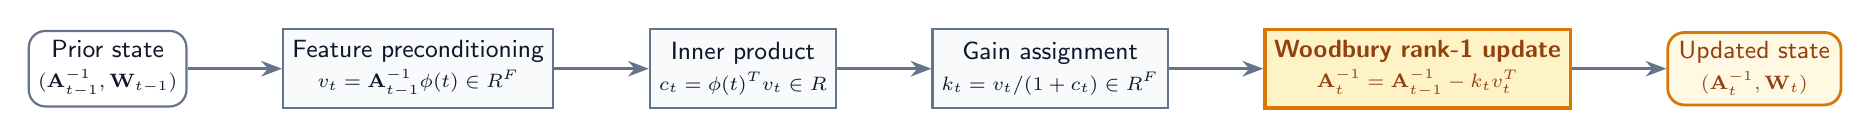
\begin{tikzpicture}[
    font=\sffamily\small,
    node distance=1.0cm and 1.2cm,
    operation/.style={rectangle, draw=neutralstroke, fill=neutralbg, text=neutraltext, minimum height=1.0cm, minimum width=2.2cm, align=center, line width=0.8pt},
    proposed_op/.style={rectangle, draw=accentstroke, fill=accentbg, text=accenttext, minimum height=1.0cm, minimum width=2.4cm, align=center, line width=1.2pt, font=\sffamily\bfseries\small},
    tensor/.style={rounded corners=6pt, draw=neutralstroke, fill=white, text=neutraltext, minimum height=0.9cm, minimum width=2.0cm, align=center, line width=0.8pt},
    proposed_tensor/.style={rounded corners=6pt, draw=accentstroke, fill=accentbg!50, text=accenttext, minimum height=0.9cm, minimum width=2.2cm, align=center, line width=1.0pt},
    arrow/.style={-{Stealth[scale=1.0]}, line width=1.0pt, draw=neutralstroke},
    aux_arrow/.style={-{Stealth[scale=1.0]}, line width=1.0pt, draw=accentstroke, dashed}
]

    % State at t-1
    \node[tensor] (state_prev) {Prior state\\{\scriptsize $(\mathbf{A}_{t-1}^{-1}, \mathbf{W}_{t-1})$}};

    % Step 1: Preconditioned feature
    \node[operation, right=of state_prev] (step1) {Feature preconditioning\\{\scriptsize $v_t = \mathbf{A}_{t-1}^{-1} \phi(t) \in \mathbb{R}^F$}};

    % Step 2: Inner product
    \node[operation, right=of step1] (step2) {Inner product\\{\scriptsize $c_t = \phi(t)^T v_t \in \mathbb{R}$}};

    % Step 3: Kalman gain
    \node[operation, right=of step2] (step3) {Gain assignment\\{\scriptsize $k_t = v_t / (1 + c_t) \in \mathbb{R}^F$}};

    % Step 4: Woodbury update (PROPOSED CONTRIBUTION)
    \node[proposed_op, right=of step3] (step4) {Woodbury rank-1 update\\{\scriptsize $\mathbf{A}_t^{-1} = \mathbf{A}_{t-1}^{-1} - k_t v_t^T$}};

    % State at t
    \node[proposed_tensor, right=of step4] (state_curr) {Updated state\\{\scriptsize $(\mathbf{A}_t^{-1}, \mathbf{W}_t)$}};

    % Arrows
    \draw[arrow] (state_prev) -- (step1);
    \draw[arrow] (step1) -- (step2);
    \draw[arrow] (step2) -- (step3);
    \draw[arrow] (step3) -- (step4);
    \draw[arrow] (step4) -- (state_curr);

\end{tikzpicture}
\end{document}
